\chapter[Aula 10]{Medida Produto e o Teorema de Fubini}
\chaptermark{}

\section{Espaço Produto}

Considere $(X, \mathscr{X})$ e $(Y, \mathscr{Y})$ espaços mensuráveis. 
Já que o produto cartesiano de $\sigma$-álgebras não 
é necessariamente uma $\sigma$-álgebra, 
a construção mais simples que nos resta é 
considerar em $X\times Y$ a $\sigma$-álgebra gerada pelos
{\it retângulos mensuráveis}, isto é, a $\sigma$-álgebra gerada
pela coleção 
$\mathscr{R}=\{ A\times B:\ A\in \mathscr{X}, B\in \mathscr{Y}\}.$ 
A $\sigma$-álgebra gerada por $\mathscr{R}$ 
é conhecida como $\sigma$-álgebra produto e 
usamos a seguinte notação $\mathscr{X}\times \mathscr{Y}$
para nos referirmos a esta $\sigma$-álgebra.



\begin{proposicao}\label{Prod. 1}
Sejam $(X, \mathscr{X})$ e $(Y, \mathscr{Y})$ espaços mensuráveis e 
$\mathscr{X}\times \mathscr{Y}$ a sigma-álgebra produto em $X\times Y$.
Então as seguintes afirmações são verdadeiras:
\begin{itemize}
\item[a)] Se $E\in \mathscr{X}\times \mathscr{Y}$ então, para cada $x\in X$ fixado,
o conjunto $[y: (x,y)\in E]:=\{y\in Y: (x,y)\in E\}$ é $\mathscr{Y}$-mensurável. 
De modo análogo, fixado $y\in Y$, 
o conjunto $[x:(x,y)\in E]:=\{x\in X: (x,y)\in E\}$ 
é $\mathscr{X}$-mensurável.



\item[b)] Se $f:X\times Y\to \mathbb{R}$ é uma função $\mathscr{X}\times \mathscr{Y}$ mensurável 
então, para cada $x\in X$ fixado, a função $y\mapsto f(x,y)$ é $\mathscr{Y}$-mensurável. De 
modo análogo, para cada $y\in Y$ fixo, a função $x\mapsto f(x,y)$ é $\mathscr{X}$-mensurável.
\end{itemize}
\end{proposicao}


\begin{proof}
\emph{Prova do item a)}. Fixe $x\in X$ e considere a aplicação  
$T_x:Y\to X\times Y$ dada por $T_x(y)=(x,y)$.
Note que se $E=A\times B\in \mathscr{X}\times \mathscr{Y}$
é um retângulo mensurável então $T_{x}^{-1}E=B~\textnormal{ou}~\varnothing$ 
dependendo apenas se 
$A$ contém ou não o ponto $x$.  

\begin{figure}
\centering
\vspace*{-0.7cm}
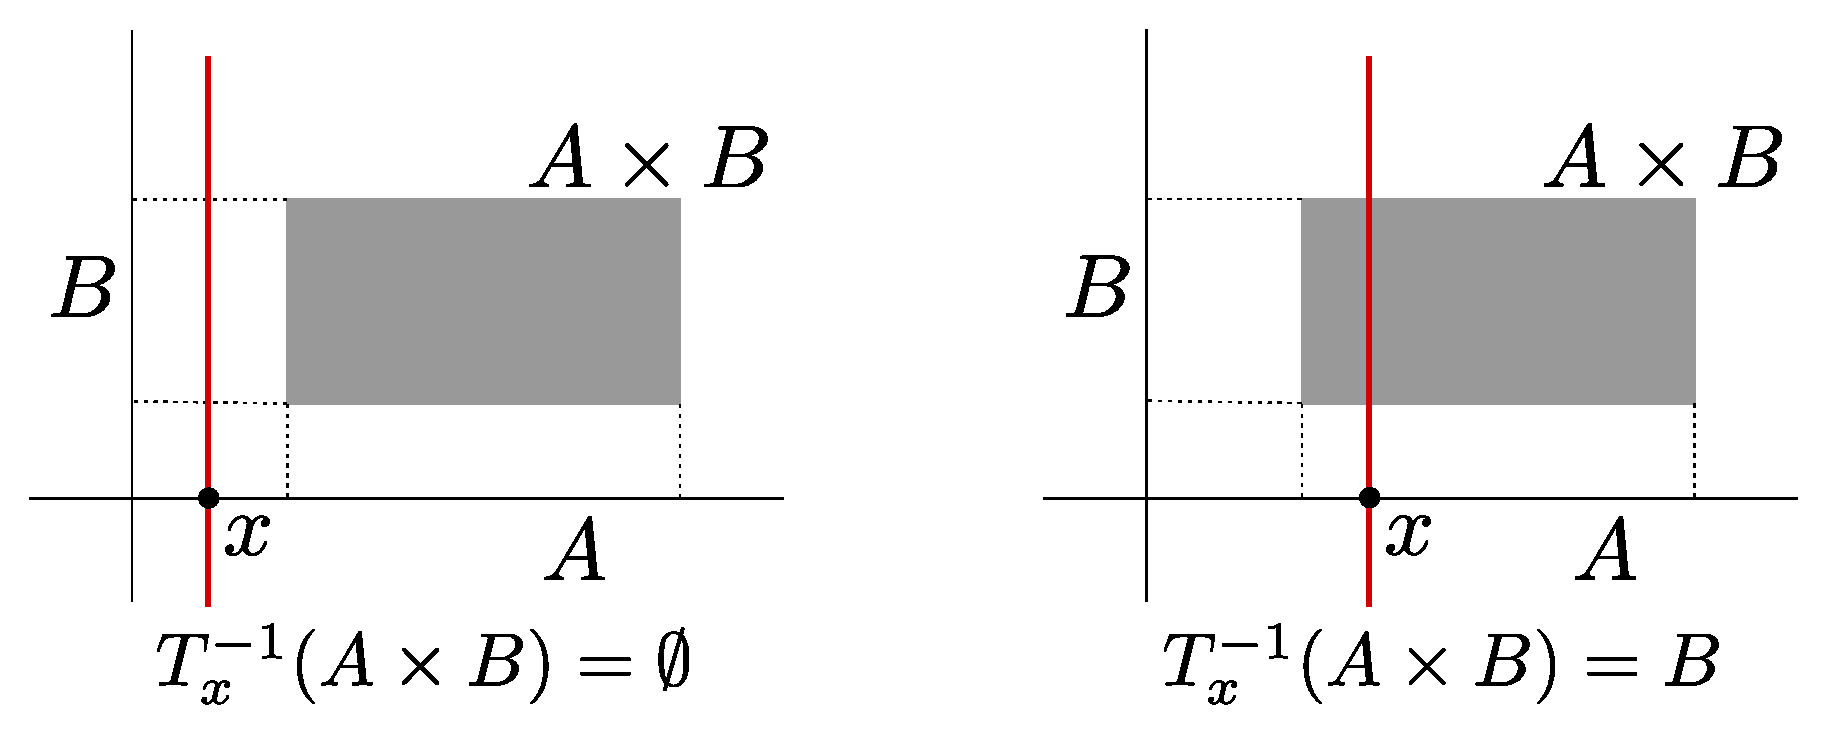
\includegraphics[scale=0.33]{Figuras/fig-medida-produto-aula10}
\caption{}
\label{medida-produto-1}
\end{figure}

De qualquer forma 
em ambas situações temos que $T_x^{-1}E\in \mathscr{Y}$.
Para mostrar que a afirmação também é válida para um conjunto 
$E$ arbitrário de $\mathscr{X}\times \mathscr{Y}$, 
basta notar que $[y: (x,y)\in E] = T^{-1}_{x}(E)$ e 
usar o seguinte exercício
\begin{exercicio}
	Sejam $(\Omega',\mathcal{F}')$ e $(\Omega,\mathcal{F})$
	dois espaços mensuráveis e $T:\Omega'\to\Omega$ uma função. 
	Suponha que $\mathcal{F}= \sigma(\mathscr{R})$
	para alguma coleção $\mathscr{R}$ de subconjuntos de $\Omega$.
	Se para todo $R\in \mathscr{R}$ temos $T^{-1}(R)\in \mathcal{F}'$
	então $T^{-1}(E)\in \mathcal{F}'$ para todo $E\in \mathcal{F}$.
\end{exercicio}
%
A prova de que $[x: (x,y)\in E]$ é $\mathscr{X}$-mensurável é feita de 
forma completamente análoga considerando a aplicação 
$T_y:X\to X\times Y$, dada por $T_y(x)=(x,y)$.

\bigskip
\noindent \emph{Prova do item b)}.  
Fixado $x\in X$ podemos observar que a aplicação $y\mapsto f(x,y)$
é dada por $f\circ T_{x}$, onde $T_x:Y\to X\times Y$ é a aplicação 
definida na prova do item a). Já que $f$ é $\mathscr{X}\times\mathscr{Y}$-mensurável
temos do item a) para qualquer boreliano $B\in \mathscr{B}(\mathbb{R})$ que 
$(f\circ T_x)^{-1}(B)= T^{-1}_x(f^{-1}(B)) \in \mathscr{Y}$.
Mostrando que $y\mapsto f(x,y)$ é $\mathscr{Y}$-mensurável para qualquer 
$x\in X$ fixado. A prova de que $x\mapsto f(x,y)$ é $\mathscr{X}$-mensurável 
para qualquer $y\in Y$ fixado é feita de maneira análoga.
\end{proof}


\begin{observacao}
Os conjunto $[y: (x,y)\in E]$ e $[x: (x,y)\in E]$ 
são chamados de seções de $E$ determinadas por $x$ e 
por $y$, respectivamente. Do mesmo modo as funções $f(x, \cdot)$ e $f(\cdot, y)$ 
são chamadas as seções de $f$ determinadas por $x$ e por $y$ respectivamente.
\end{observacao}



\section{Medida Produto}
Sejam $(X, \mathscr{X}, \mu)$ e $(Y, \mathscr{Y}, \nu)$
espaços de medida. 
O objetivo nesta seção é definir uma medida $\pi$ no produto cartesiano 
$\mathscr{X}\times \mathscr{Y}$ tal que para todo 
retângulo mensurável $E=A\times B$ temos  
$\pi(E)=\mu(A)\nu(B)$. 
A seguir vamos ver que se 
$ \mu$ e $\nu$ são medidas $\sigma$-finitas então 
existe uma única medida com a propriedade mencionada acima, 
que será chamada de \emph{medida produto} e além do mais 
ela é a única medida em $\mathscr{X}\times\mathscr{Y}$ 
com tal propriedade.
\medskip
 

Sejam $(X, \mathscr{X}, \mu)$ e $(Y, \mathscr{Y}, \nu)$
espaços de medida com $\mu$ e $\nu$ finitas. 
Segue  da Proposição (\ref{Prod. 1}) que dado
$E\in \mathscr{X}\times \mathscr{Y}$ a função 
$x\mapsto \nu([y:(x,y)\in E])$ está bem definida 
para todo $x\in X$ e assume valores no intervalo $[0, \infty)$.
Analogamente para todo $y\in Y$ temos que a 
aplicação $y\mapsto \mu([x:(x,y)\in E])$ 
está bem definida e também toma valores em $[0, \infty)$.
Seja $\mathscr{L}$ a coleção de todos os subconjuntos 
$E\in \mathscr{X}\times \mathscr{Y}$
para os quais as funções acima são $\mathscr{X}$ e $\mathscr{Y}$-mensuráveis,
respectivamente.

\begin{proposicao}\label{Mens. Prod}
A coleção $\mathscr{L}$, definida no parágrafo acima, 
coincide com a $\sigma$-álgebra  $\mathscr{X}\times \mathscr{Y}$.
\end{proposicao}
\begin{proof}
Vamos mostrar inicialmente que $\mathscr{L}$ 
é um $\lambda$-sistema. 
Primeiro vamos mostrar que $E=X\times Y\in \mathscr{L}$.
Para verificar que a afirmação é verdadeira 
basta observar que $\nu([y:(x,y)\in X\times Y])=\nu(Y) < \infty$, 
para todo $x\in X$. Já que a função 
$x\mapsto \nu([y:(x,y)\in X\times Y])\equiv \nu(Y)$ 
é constante ela é claramente $\mathscr{X}$-mensurável.

Vamos mostrar agora que a coleção $\mathscr{L}$ é fechada 
para complementação. Seja $E\in \mathscr{L}$.
Usando propriedades elementares de medida 
podemos afirmar que 
\[ 
\nu( [y:(x,y)\in E^c] )=\nu(Y)-\nu([y:(x,y)\in E]).
\]
Já que o lado direito da igualdade acima 
define uma função mensurável com 
respeito a $\mathscr{X}$ pois,  
qualquer função constante é $\mathscr{X}$-mensurável
e $\nu([y:(x,y)\in E)$ é $\mathscr{X}$-mensurável por hipótese,
segue que $x\to \nu( [y:(x,y)\in E^c] )$ é $\mathscr{X}$-mensurável. 
Este fato mostra que $\mathscr{L}$ é uma coleção fechada para complementação.

Vamos mostrar agora que se $\{ E_n \}_{n\in\mathbb{N}}$ 
é uma sequência infinita de conjuntos mutuamente disjuntos em $\mathscr{L}$,
então $\cup_{n\geq 1} E_n\in \mathscr{L}$. 
Para provar este fato primeiro observamos que 
$
[y:(x,y)\in \cup_{n\geq 1}E_n ] 
= 
\cup_{n \geq 1}  
[y:(x,y)\in E_n ]
$, sendo a sequência de conjuntos que aparece no lado direito
desta igualdade mutuamente disjunta.  
Daí segue da $\sigma$-aditividade de $\nu$ que
\[
\nu \big( [y:(x,y)\in \cup_{n\geq 1}E_n ] \big)
= 
\sum_{n \geq 1}  
\nu ([y:(x,y)\in E_n ])
\]
Por hipótese temos que, para cada $n\geq 1$, 
a aplicação $x\mapsto \nu ([y:(x,y)\in E_n ])$ 
é $\mathscr{X}$-mensurável. 
Assim segue do Lema \ref{inf-sup-func-mensuraval-eh-mensuravel} 
(olhando para a séria acima, como limite da sequência das somas parciais) 
que $x\mapsto \nu \big( [y:(x,y)\in \cup_{n\geq 1}E_n ] \big)$ é 
$\mathscr{X}$-mensurável. 
Este fato encerra a prova de que $\mathscr{L}$ é um $\lambda$-sistema.
 
Agora vamos provar que $\mathscr{L}$ contém o $\pi$-sistema 
dos retângulos mensuráveis $\mathscr{R}$. 
De fato, se $E=A\times B\in \mathscr{R}$ 
vimos na prova da Proposição \ref{Prod. 1} que 
\[
[y:(x,y)\in A\times B ]
=
\begin{cases}
\emptyset,&\ \text{se}\ x\notin A;
\\
B,&\ \text{se}\ x\in A. 
\end{cases}
\] 
Desta igualdade segue que
$\nu([y:(x,y)\in A\times B ]) = 1_A(x)\nu(B)$ 
e desta forma a função $x\mapsto \nu([y:(x,y)\in A\times B ])$ 
é $\mathscr{X}$-mensurável, para qualquer $A\times B\in\mathscr{R}$
mostrando que este $\pi$-sistema está contido em $\mathscr{L}$. 

Pelo Teorema $\pi$-$\lambda$ de Dynkin 
temos finalmente que $\mathscr{X}\times \mathscr{Y}= \sigma(\mathscr{R})\subset \mathscr{L}\subset \mathscr{X}\times \mathscr{Y}$ concluindo a demonstração.
\end{proof}


\bigskip


\subsubsection{Contrução da Medida Produto - Caso de Medidas Finitas}
Vamos apresentar a seguir a construção da medida produto no caso 
em que ambos espaços $(X,\mathscr{X},\mu)$ e $(Y,\mathscr{Y},\nu)$
são espaços de medida finita. 
Primeiro observamos que a mensurabilidade 
garantida pela Proposição \ref{Prod. 1},
junto com a não-negatividade das funções
$x\mapsto \nu([y:(x,y)\in E ])$ e $y\mapsto \mu([x:(x,y)\in E ])$
nos permite definir as seguintes 
funções de conjunto $\pi_1$ e $\pi_2$, como segue
\begin{equation}\label{M.Prod. 1}
\pi_1(E)=\int_X \nu([y:(x,y)\in E ])\, d\mu(x),~~~~~E \in \mathscr{X}\times \mathscr{Y}
\end{equation}
e 
\begin{equation}\label{M. Prod. 2}
\pi_2(E)=\int_Y \mu([x:(x,y)\in E ])\, d\nu(y),~~~~~E \in \mathscr{X}\times \mathscr{Y}.
\end{equation}

Como estamos assumindo que 
$(X,\mathscr{X},\mu)$ e $(Y,\mathscr{Y},\nu)$
são espaços de medida finita é imediato verificar 
que tanto $\pi_1$ quanto $\pi_2$ 
são funções de conjunto finitas em $\mathscr{X}\times \mathscr{Y}$.

Afirmamos que $\pi_1$ e $\pi_2$ definem medidas sobre 
$(X\times Y,\mathscr{X}\times\mathscr{Y})$. 
Vamos apresentar apenas a prova de que $\pi_1$ é uma medida,
já que a prova deste fato para $\pi_2$
é completamente análoga.


É fácil ver que $\pi_1(\emptyset)=0$ e que $\pi_1(E)\geq 0$ 
para todo $E\in \mathscr{X}\times\mathscr{Y}$. Para provar
que $\pi_1$ é $\sigma$-aditiva, considere  
$\{E_n\}_{n\geq 1}$ uma sequência em $\mathscr{X}\times\mathscr{Y}$
de conjuntos mutuamente disjuntos.
Usando que $\nu$ é uma medida em $Y$ temos que 
\[
\nu([y:(x,y)\in \cup_{j=1}^n E_j ])
=
\sum_{j=1}^n \nu([y:(x,y)\in E_j ])
:=\varphi_n(x).
\]
Pela continuidade da medida $\nu$ podemos afimar que 
$\varphi_n(x) \to \nu([y:(x,y)\in \cup_{j\geq 1} E_j ])$,
para todo $x\in X$. Já que $\{\varphi_n\}_{n\in\mathbb{N}}$ é 
uma sequência de funções monótona, $\mathscr{X}$-mensuráveis 
e não-negativas segue do Teorema da Convergência
Monótona que 
\begin{align*}
\pi_1(\cup_{j\geq 1} E_j)
&=
\int_X \nu([y:(x,y)\in \cup_{j\geq 1} E_j ])\, d\mu(x)
\\
&=
\int_X \lim_{n\to\infty} \varphi_n(x)\, d\mu(x)
\\
&=
\lim_{n\to\infty}\int_X \varphi_n(x)\, d\mu(x)
\\
&=
\lim_{n\to\infty}\int_X \sum_{j=1}^n \nu([y:(x,y)\in E_j ])\, d\mu(x)
\\
&=
\lim_{n\to\infty}\sum_{j=1}^n\int_X \nu([y:(x,y)\in E_j ])\, d\mu(x)
\\
&=
\lim_{n\to\infty}\sum_{j=1}^n \pi_1(E_j)
\\
&=
\sum_{j=1}^{\infty} \pi_1(E_j).
\end{align*}



Para o caso especial em que $E=A\times B\in\mathscr{X}\times \mathscr{Y}$  
é um retângulo mensurável, 
temos que  $\nu([y:(x,y)\in E ])=1_A(x)\nu(B)$ 
e 
$\mu([x:(x,y)\in E ])=1_B(y)\mu(A)$, e desta forma temos 
\[ 
\pi_1(A\times B)=\mu(A)\nu(B)=\pi_2(A\times B).
\]
Assim as medidas $\pi_1$ e $\pi_2$ coincidem no $\pi$-sistema $\mathscr{R}$.  
A menos de uma 
normalização por um fator de $\mu(X)\nu(Y)$, podemos supor que
ambas $\pi_1$ e $\pi_2$ são medidas de probabilidade e 
aplicar o Corolário \ref{cor-uni-medidas-teo-pi-lambda} que garante
a igualde $\pi_1 = \pi_2$ em $\sigma(\mathscr{R})=\mathscr{X}\times\mathscr{Y}$. 














\subsubsection{Construção da Medida Produto - Caso de Medidas $\sigma$-finitas}


Próximo passo é generalizar a construção feita
acima para o caso que ambos espaços 
$(X,\mathscr{X},\mu)$ e $(Y,\mathscr{Y},\nu)$
são espaços de medida $\sigma$-finitos.

Como estamos assumindo que os espaços 
$(X,\mathscr{X},\mu)$ e $(Y,\mathscr{Y},\nu)$
são $\sigma$-finitos, sabemos 
que existem sequências $\{A_m\}_{m\in\mathbb{N}}$
e $\{B_n\}_{n\in\mathbb{N} }$ em $\mathscr{X}$ e $\mathscr{Y}$, respectivamente 
tais que $\cup_{m\geq 1} A_m=X$ e 
$\cup_{m\geq 1} B_n = Y$ e além do mais $\mu(A_m)<\infty$
e $\nu(B_n)<\infty$ para todo $m,n\in\mathbb{N}$.
Sem perda de generalidade, podemos supor que ambas sequências
são crescentes, i.e., $A_{m}\subset A_{m+1}$ e
$B_{n}\subset B_{n+1}$. 
Defina para cada $m,n\in\mathbb{N}$ as seguintes 
medidas $\mu_m(A)=\mu(A\cap A_m)$ e 
$\nu_n(B)=\nu_n(B\cap B_n)$.

Pelos resultados da seção anterior podemos definir em
$(X\times Y,\mathscr{X}\times\mathscr{Y})$ as seguintes
medidas
\begin{equation}\label{M.Prod.1mn}
\pi_1^{m,n}(E)
=
\int_X \nu_n([y:(x,y)\in E ])\, d\mu_m(x),~~~~~E \in \mathscr{X}\times \mathscr{Y}
\end{equation}
e 
\begin{equation}\label{M. Prod.2mn}
\pi_2^{m.n}(E)
=
\int_Y \mu_m([x:(x,y)\in E ])\, d\nu_n(y),~~~~~E \in \mathscr{X}\times \mathscr{Y}
\end{equation}
e vimos que ambas medidas coincidem em 
$\mathscr{X}\times \mathscr{Y}$.
A ideia é mostrar que existem os seguintes limites:
\[
\lim_{m\to\infty}
\left( \lim_{n\to\infty} \pi_1^{m,n}(E) \right)
:=\pi_1(E)
\quad\text{e}\quad
\lim_{n\to\infty}
\left( \lim_{m\to\infty} \pi_2^{m,n}(E) \right)
:=\pi_2(E),
\]
onde $\pi_1$ e $\pi_2$ são medidas $\sigma$-finitas 
com $\pi_1=\pi_2$ em $\mathscr{X}\times\mathscr{Y}$.

Vamos apresentar o argumento da existência do primeiro limite
acima. Sejam $m,n\in\mathbb{N}$ fixado. Por definição temos 
que 
\begin{align*}
\pi_1^{m,n}(A)
&=
\int_X \nu_n([y:(x,y)\in E ])\, d\mu_m(x)
\end{align*}
Procedendo como na seção anterior podemos ver que 
para qualquer $E\in\mathscr{X}\times\mathscr{Y}$
a aplicação $x\mapsto \nu_n([y:(x,y)\in E ])$ 
define uma função $\mathscr{X}$-mensurável para 
cada $n\in\mathbb{N}$, vamos denotar esta aplicação 
por $\varphi_n$. Note que 
\begin{align*}
\varphi_n(x):=
\nu_n([y:(x,y)\in E ])
&=
\nu([y:(x,y)\in E ]\cap B_n)
\\
&=
\nu([y:(x,y)\in E \cap X\times B_n])
\\
&\leq 
\nu([y:(x,y)\in E \cap X\times B_{n+1}])
\\
&= 
\nu([y:(x,y)\in E]\cap B_{n+1})
\\
&=
\varphi_{n+1}(x).
\end{align*}
Já que $\cup_{n\geq 1} B_n= Y$ segue da continuidade da probabilidade 
que $\varphi_n(x)\uparrow \nu([y:(x,y)\in E])$, para todo 
$x\in X$. Fixado $m\in\mathbb{N}$ 
segue do Teorema da Convergência Monótona que 
o seguinte limite existe 
\begin{align*}
\lim_{n\to\infty}\pi_1^{m,n}(E)
&=
\lim_{n\to\infty}
\int_X \nu_n([y:(x,y)\in E ])\, d\mu_m(x)
\\
&=
\int_X \lim_{n\to\infty} \nu_n([y:(x,y)\in E\cap X\times B_{n} ])\, d\mu_m(x)
\\
&=
\int_X \nu([y:(x,y)\in E ])\, d\mu_m(x)
\end{align*}

É fácil ver para qualquer função $\mathscr{X}$-mensurável $g:X\to [0,+\infty]$ que 
\[
\int_X g \,d\mu_n = \int_{A_m} g\, d\mu.
\]
Usando este fato na igualdade obtida acima, conjuntamente 
com o Teorema da Convergência Monótona concluímos que
existe o seguinte limite 
\begin{align*}
\lim_{m\to\infty} \lim_{n\to\infty}\pi_1^{m,n}(E)
&=
\lim_{m\to\infty}\int_X \nu([y:(x,y)\in E ])\, d\mu_m(x)
\\
&=
\lim_{m\to\infty}\int_{X\cap A_m} \nu([y:(x,y)\in E ])\, d\mu(x)
\\
&=
\int_{X} \nu([y:(x,y)\in E ])\, d\mu(x).
\end{align*}
De forma análoga temos que 
\begin{align*}
\lim_{n\to\infty} \lim_{m\to\infty}\pi_2^{m,n}(E)
&=
\int_{Y} \mu([x:(x,y)\in E ])\, d\nu(x).
\end{align*}
Da seção anterior segue que $\pi_1^{m,n}(E)= \pi_2^{m,n}(E)$. Portanto
resta mostrar apenas que 
\begin{equation}\label{igualdade-pi1mn-pi2mn}
\lim_{m\to\infty}\lim_{n\to\infty} \pi_1^{m,n}(E)
=
\lim_{n\to\infty}\lim_{m\to\infty} \pi_1^{m,n}(E).
\end{equation}
O lado esquerdo da última igualdade foi avaliado logo acima. 
Para verificar que a última igualdade é válida basta aplicar duas vezes o
Teorema da Convergência Monótona como segue
\begin{align*}
\lim_{n\to\infty}\lim_{m\to\infty} \pi_1^{m,n}(E)
&=
\lim_{n\to\infty}\lim_{m\to\infty}
\int_X \nu_n([y:(x,y)\in E ])\, d\mu_m(x)
\\
&=
\lim_{n\to\infty}\lim_{m\to\infty}
\int_{X\cap A_m} \nu_n([y:(x,y)\in E ])\, d\mu(x)
\\
&=
\lim_{n\to\infty}
\int_{X} \nu_n([y:(x,y)\in E ])\, d\mu(x)
\\
&=
\int_{X} \nu([y:(x,y)\in E ])\, d\mu(x).
\end{align*} 

Usando a igualdade \eqref{igualdade-pi1mn-pi2mn} e os valores 
calculados destes limites segue que 
\begin{align*}
\int_{X} \nu([y:(x,y)\in E ])\, d\mu(x)
&=
\lim_{m\to\infty} \lim_{n\to\infty}\pi_1^{m,n}(E)
\\
&=
\lim_{n\to\infty} \lim_{m\to\infty}\pi_2^{m,n}(E)
\\
&=
\int_{Y} \mu([x:(x,y)\in E ])\, d\nu(x).
\end{align*}



Desta forma podemos definir uma medida 
$\pi:\mathscr{X}\times\mathscr{Y}\to [0,\infty]$ 
tal que para qualquer conjunto $E\in \mathscr{X}\times\mathscr{Y}$ 
temos 
\[
\pi(E) := \pi_1(E) = \pi_2(E)
\] 
e além do mais 
\[
	\int_{X} \nu([y:(x,y)\in E ])\, d\mu(x)
	=
	\pi_1(E)
	=
	\pi_2(E)
	=
	\int_{Y} \mu([x:(x,y)\in E ])\, d\nu(x).
\]
A medida $\pi$ possui a seguinte propriedade.
Para qualquer retângulo mensurável 
$A\times B\in \mathscr{X}\times\mathscr{Y}$ temos que 
\[
\pi(A\times B)=\mu(A)\nu(B).
\]
Uma vez que $\{A_m\times B_m: m\in \mathbb{N}\}$ é uma cobertura 
de $X\times Y$ segue da propriedade acima que 
$\pi$ é uma medida $\sigma$-finita. 
Para verificar que $\pi$ é a única medida com esta propriedade
basta notar que qualquer medida $\lambda$ satisfazendo 
$\lambda(A\times B)=\mu(A)\nu(B)$ necessariamente
coincide com $\pi$ na álgebra dos retângulos mensuráveis 
$\mathscr{R}$. Logo ambas, pelo Teorema de Carathéodory,
admitem extensão única a 
$\sigma(\mathscr{R})=\mathscr{X}\times\mathscr{Y}$ 
e portanto temos que $\pi=\lambda$.  

A medida $\pi$ é comumente chamada de \textbf{medida produto} e 
usamos a notação $\pi = \mu\times\nu$ para indicar esta medida.







\section{Teorema de Fubini}  
Sejam $(X, \mathscr{X}, \mu)$ e $(Y, \mathscr{Y}, \nu)$
espaços de medida com $\mu$ e $\nu$ medidas $\sigma$-finitas. 
Considere  na $\sigma$-álgebra
produto $\mathscr{X}\times \mathscr{Y}$ 
a medida produto $\pi = \mu\times \nu$ e 
$f:X\times Y\to \overline{\mathbb{R}}$ 
uma função $\mathscr{X}\times \mathscr{Y}$-mensurável. 
O objetivo nesta seção é encontrar condições suficientes  
sobre a função $f$ que garantam a validade
das seguintes igualdades:
\begin{equation}\label{Fubini1}
\int_{X\times Y}f d\pi
= 
\int_X\left[ \int_Y f(x,y) d\nu(y)\right] d\mu(x)
\end{equation}
e
\begin{equation}\label{Fubini2}
\int_{X\times Y}f\, d\pi
=
\int_Y\left[\int_Xf(x,y) d\mu(x)\right] d\nu(y).
\end{equation}
Seria desejável que as expressões (\ref{Fubini1}) e (\ref{Fubini2}) 
fossem válidas para todas as funções $\mathscr{X}\times\mathscr{Y}$
mensuráveis. Em geral, isto não será verdadeiro. Mas 
podemos provar a validade destas igualdades se adicionamos
à hipotese de $\mathscr{X}\times \mathscr{Y}$-mensurabilidade a 
condição de $f$ ser não-negativa. 
Este resultado é conhecido na literatura como Teorema de Tonneli. 
Se permitimos que $f$ tome valores positivos e negativos é possível  
garantir a validade de (\ref{Fubini1}) e (\ref{Fubini2}) 
assumindo a integrabilidade de $f$. Este resultado é o conhecido 
como Teorema de Fubini.




\begin{teorema}[Tonelli]\label{Tonelli}
Sejam $(X, \mathscr{X}, \mu)$ e $(Y, \mathscr{Y}, \nu)$
espaços de medida. 
Suponha que $\mu$ e $\nu$ sejam medidas $\sigma$-finitas. 
Considere na $\sigma$-álgebra produto $\mathscr{X}\times \mathscr{Y}$ 
a medida produto $\pi = \mu\times \nu$ e seja $f:X\times Y\to \overline{\mathbb{R}}$ 
uma função $\mathscr{X}\times \mathscr{Y}$-mensurável 
\textbf{não-negativa}. Nestas condições as funções 
\begin{equation}\label{sec-int-mensuraveis-teo-tonelli}
x\mapsto \int_Y f(x,y) d\nu(y)
\quad\text{e}\quad
y\mapsto \int_X f(x,y) d\mu(x)
\end{equation}
são $\mathscr{X}$ e $\mathscr{Y}$-mensuráveis, respectivamente
e além do mais valem (\ref{Fubini1}) e (\ref{Fubini2}). 
\end{teorema}





\begin{proof}
Vamos mostrar primeiro que o teorema é válido para funções da forma 
$1_E,~E\in \mathscr{X}\times \mathscr{Y}$. 
Neste caso as funções em \eqref{sec-int-mensuraveis-teo-tonelli}
são dadas por $x\mapsto \nu([y:(x,y)\in E])$ e 
$y\mapsto \mu([x:(x,y)\in E])$, respectivamente e a mensurabilidade destas 
funções com respeito as $\sigma$-álgebras $\mathscr{X}$ e $\mathscr{Y}$
é garantida pelo Proposição \ref{Mens. Prod}.

Agora vamos calcular separadamente os lados direito e esquerdo de
(\ref{Fubini1}) e (\ref{Fubini2}) e mostrar que eles coincidem.
O lado esquerdo de (\ref{Fubini1}) foi obtido na seção anterior 
e é dado por
\begin{equation}
\int_{X\times Y} 1_E\, d\pi 
=
\mu\times \nu( E)
=
\int_X \nu([y:(x,y)\in E]) d\mu(x).
\end{equation}
Por outro lado, note que para cada $x\in X$ fixado 
\[ 
1_E(x,\cdot) 
=
1_{[y:(x,y)\in E]}(\cdot)
\]
e além disto segue da Proposição \ref{Prod. 1} 
que esta função é $\mathscr{Y}$-mensurável. 
Por outro lado, temos diretamente da definição 
da integral de Lebesgue que
\begin{equation}
\int_X
\left[ \int_Y 1_E(x,y)\, d\nu(y)\right] d\mu(x)
= 
\int_X \nu([y:(x,y)\in E]) d\mu(x)
\end{equation}
e portanto (\ref{Fubini1}) está provada. 
De modo análogo verificamos que vale (\ref{Fubini2}). 

Da linearidade da integral e do exposto acima 
concluímos a mensurabilidade das funções em
\eqref{sec-int-mensuraveis-teo-tonelli} com
respeito a suas respectivas $\sigma$-álgebras
e também que as igualdades (\ref{Fubini1}) e (\ref{Fubini2})  
são válidas para quaisquer funções simples desde que 
sejam $\mathscr{X}\times\mathscr{Y}$-mensuráveis. 
O próximo passo é ``aproximar'' $f$ por uma sequência
monótona não-decrescente de funções simples. 
Como estamos assumindo que $f$ é não-negativa, 
esta aproximação pode ser feita 
via o Teorema \eqref{teo:aproximacao-monotona-por-func-simples}.
Já que o limite pontual de funções mensuráveis é uma 
função mensurável 
(Corolário \ref{cor-lim-mensuravel-eh-mensuravel})
basta usar o Teorema de Convergência Monótona 
para verificar a mensurabilidade de \ref{sec-int-mensuraveis-teo-tonelli}
e a validade de (\ref{Fubini1}) e (\ref{Fubini2}) 
para qualquer função $f$ não-negativa e 
$\mathscr{X}\times\mathscr{Y}$-mensurável.
\end{proof}




\begin{teorema}[Fubini]
Sejam $(X, \mathscr{X}, \mu)$ e $(Y, \mathscr{Y}, \nu)$
espaços de medida com $\mu$ e $\nu$ medidas $\sigma$ finitas. 
Seja $\pi= \mu\times \nu$ a medida produto definida
em $\mathscr{X}\times \mathscr{Y}$  e 
$f:X\times Y\to \overline{\mathbb{R}}$ uma função 
$\mathscr{X}\times \mathscr{Y}$-mensurável tal que 
$|f|$ seja integrável. 
Nestas condições as funções 
\begin{equation}\label{sec-int-mensuraveis-teo-tonelli}
x\mapsto \int_Y f(x,y) d\nu(y)
\quad\text{e}\quad
y\mapsto \int_X f(x,y) d\mu(x)
\end{equation}
são $\mathscr{X}$ e $\mathscr{Y}$-mensuráveis, respectivamente
e além do mais valem (\ref{Fubini1}) e (\ref{Fubini2}).
\end{teorema}

\begin{proof}
Já que $|f|$ é uma função não-negativa 
e integrável, temos pelo Teorema de Tonelli que 
\begin{eqnarray}\label{Fubini 2}
\int_X \left[ \int_Y |f(x,y)| \,d\nu(y)  \right] d\mu(x)
=
\int_{X\times Y}|f|\,  d\pi<\infty.
\end{eqnarray}
Observe que a função $\varphi:X\to \mathbb{R}$ 
definida por $\varphi(x)=\int_Y |f(x,y)| d\nu(y)$ 
satisfaz  $\varphi(x)<\infty$ $\mu$-q.t.p.  
Seja $A_0= \{ x\in X: \varphi(x)<\infty \}$.
Então temos que 
$\mu(X\setminus A_0)=0
$ e para todo $x\in A_0$ vale a seguinte igualdade  
\begin{equation}
\int_Y f(x,y)\, d\nu(y)
=
\int_{Y}f^{+}(x,y)\, d\nu(y)
-
\int_Y f^{-}(x,y)\, d\nu(y).
\end{equation}
Desta forma temos que  

\begin{align*}
\hspace{3em}&\hspace{-5em}
\int_X  \left[ \int_Y f(x,y)\, d\nu(y) \right] d\mu(x)
\\[0.3cm]
&=
\int_{A_0}
\left[ \int_Y f(x,y)d\nu\right] d\mu(x)
+
\underbrace{
\int_{X\setminus A_0} 
\left[
\int_Y f(x,y)\, d\nu(y) d\mu(x)
\right]
}_{=0}
\\[0.4cm]
%
%
&=
\int_{A_0}\left[
\int_{Y}f^{+}(x,y)\, d\nu(y)
\right] d\mu(x)
-
\int_{A_0}\left[
\int_{Y}f^{-}(x,y)\, d\nu(y)
\right] d\mu(x)
\\[3mm]
%
%
&=
\int_{X}\left[
\int_{Y}f^{+}(x,y)\, d\nu(y) 
\right] d\mu(x)
-
\int_{X}\left[ 
\int_{Y}f^{-}(x,y)d\nu(y)
\right] d\mu(x)
\\[3mm]
%
%
&=
\int_{X\times Y}
f^{+}\, d\pi 
-
\int_{X\times Y}
f^{-}\, d\pi
\\[3mm]
%
%
&=
\int_{X\times Y}
f\, d\pi,
\end{align*}
onde da antepenúltima para a penúltima linha 
usamos o Teorema de Tonelli.
\end{proof}


\subsubsection{Contra-exemplos}


\noindent\textbf{Contra-exemplo 1.} 
Vamos mostrar que não podemos remover do enunciado do 
Teorema de Fubini a hipótese de $|f|$ ser integrável. 
Para isso considere uma sequência 
$\{\delta_n\}_{n\in\mathbb{N} }\subset [0,1]$ 
com $0=\delta_0<\delta_1<\cdots <\delta_n<\cdots $ 
e $\delta_n\to 1$. 
Seja $(g_n)$ uma sequência de funções reais 
contínuas positivas 
definidas em $[0,1]$ onde cada $g_n$ 
tem suporte em $(\delta_n,\delta_{n+1})$ e satisfaz 
$\int_{0}^{1}g_n(t)dt=1$. 
Considere a função  $f:[0,1]\times [0,1]\to \mathbb{R}$
definida por
$$
f(x,y)=\sum_{n=1}^{\infty}[(g_n(x)-g_{n-1}(x)]g_n(y)
$$
note que $f$ está bem definida, de fato, 
para cada par $(x,y)$ no máximo um dos termos da 
série que define $f$ é não nulo. 
Também não temos problemas quanto à 
mensurabilidade de $f$. Veja, 
$$
\int_{0}^1(\int_{0}^{1}f(x,y)dy)dx.
$$
